\documentclass[12pt, aspectratio=169]{beamer}

\input{../header}
\usepackage{booktabs}

\title{Types of Hypothesis Tests}
\author{Md. Aminul Islam Shazid}
\date{}


\begin{document}
    {
        \setbeamertemplate{footline}{}
        \addtocounter{framenumber}{-2}

        \begin{frame}
            \titlepage
        \end{frame}

        \begin{frame}{Outline}
            \vfill
            \tableofcontents[subsectionstyle=hide]
            \vfill
        \end{frame}
    }

    \section{Test about a Single Mean}


    \begin{frame}{Test about a Single Mean --- Choosing the Test}
        \begin{center}
            \begin{tabular}{lll}
                \toprule
                \textbf{Criteria} & \textbf{Test} & \textbf{Test Statistic} \\
                \midrule
                $\sigma$ known & $Z$-test &
                    $Z_{\text{cal}} = \dfrac{\bar{x} - \mu_0}{\sigma/\sqrt{n}} \sim N(0,1)$ \\[1.2em]
                $\sigma$ unknown, $n \geqslant 30$ & $Z$-test &
                    $Z_{\text{cal}} = \dfrac{\bar{x} - \mu_0}{s/\sqrt{n}} \sim N(0,1)$ \\[1.2em]
                $\sigma$ unknown, $n < 30$ & $t$-test &
                    $t_{\text{cal}} = \dfrac{\bar{x} - \mu_0}{s/\sqrt{n}} \sim t_{n-1}$ \\
                \bottomrule
            \end{tabular}
        \end{center}

        \vspace{0.5em}

        \begin{itemize}
            \item All three test statistics are computed the same way; only the
                \textbf{sampling distribution} and critical values differ
        \end{itemize}
    \end{frame}


    \begin{frame}{Test about a Single Mean --- Example (Large Sample, $Z$-test)}
        \textbf{Problem:} The mean length of a chocolate bar is 43\,mm.
        An engineering team selects a random sample of 40 bars and finds a
        mean of 41.5\,mm with $s = 1.8$.
        At $\alpha = 0.01$, has the mean length changed?

        \vspace{0.8em}

        Let $\mu = $ mean length of the bars.

        \[
            H_0: \mu = 43 \quad \text{vs} \quad H_A: \mu \neq 43
        \]

        \vspace{0.5em}

        \textbf{Assumptions:} Population is approximately normal; $\sigma$ unknown,
        estimated from large sample ($n = 40$).
    \end{frame}


    \begin{frame}{Test about a Single Mean --- Solution ($Z$-test)}
        \begin{columns}
            \begin{column}{0.55\textwidth}
                \textbf{Test statistic:}
                \[
                    Z_{\text{cal}} = \frac{\bar{x} - \mu_0}{s/\sqrt{n}}
                    = \frac{41.5 - 43}{1.8/\sqrt{40}} = -5.27
                \]
                \textbf{Critical value:} $Z_{0.005} = \pm 2.57$

                \vspace{0.5em}

                \textbf{Decision:} Since $Z_{\text{cal}} = -5.27 < -2.57$,
                we \textbf{reject} $H_0$ at 1\% level of significance.

                \vspace{0.5em}

                \textbf{P-value:} \(p = 2\,P(Z \geqslant 5.27) \approx 0.000\)

                \vspace{0.5em}

                Since $p < \alpha = 0.01$, we reject $H_0$.
                There is extremely strong evidence that the mean length has changed.
            \end{column}
            \begin{column}{0.45\textwidth}
                % R code to generate the plot:
                % library(ggplot2)
                % alpha <- 0.01
                % z_crit <- qnorm(1 - alpha/2)   # 2.576
                % z_cal  <- -5.27
                %
                % x  <- seq(-6, 6, length.out = 600)
                % df <- data.frame(x = x, y = dnorm(x))
                %
                % ggplot(df, aes(x, y)) +
                %   geom_line() +
                %   geom_area(data = subset(df, x <= -z_crit),
                %             aes(x, y), fill = "firebrick", alpha = 0.4) +
                %   geom_area(data = subset(df, x >=  z_crit),
                %             aes(x, y), fill = "firebrick", alpha = 0.4) +
                %   geom_vline(xintercept = z_cal, linetype = "dashed",
                %              colour = "blue") +
                %   annotate("text", x = z_cal - 0.4, y = 0.15,
                %            label = expression(Z[cal] == -5.27),
                %            hjust = 1, colour = "blue") +
                %   annotate("text", x = -z_crit - 0.1, y = 0.02,
                %            label = "-2.57", hjust = 1) +
                %   annotate("text", x =  z_crit + 0.1, y = 0.02,
                %            label =  "2.57", hjust = 0) +
                %   labs(x = "Z", y = "") +
                %   theme_classic()
                %
                % ggsave("plots/single-mean-z-test.pdf", width = 4, height = 3)
                \begin{center}
                    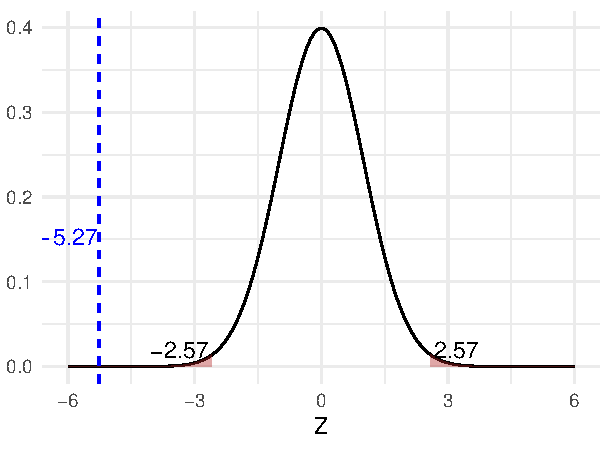
\includegraphics[width=\textwidth]{plots/single-mean-z-test.pdf}
                \end{center}
            \end{column}
        \end{columns}
    \end{frame}


    \begin{frame}{Test about a Single Mean --- Example (Small Sample, $t$-test)}
        \textbf{Problem:} It is claimed that the mean weight of teens in a city
        is 35\,kg. A sample of $n = 10$ teens yields $\bar{x} = 40.1$\,kg,
        $s = 4.2$\,kg. At $\alpha = 0.05$, does the mean weight differ from 35\,kg?

        \vspace{0.8em}

        Let $\mu = $ mean weight of the teens.

        \[
            H_0: \mu = 35 \quad \text{vs} \quad H_A: \mu \neq 35
        \]

        \vspace{0.5em}

        \textbf{Assumptions:} Population is normally distributed; $\sigma$ unknown,
        estimated from a small sample ($n = 10 < 30$) $\Rightarrow$ use $t$-test.
    \end{frame}


    \begin{frame}{Test about a Single Mean --- Solution ($t$-test)}
        \begin{columns}
            \begin{column}{0.55\textwidth}
                \textbf{Test statistic:}
                \[
                    t_{\text{cal}} = \frac{\bar{x} - \mu_0}{s/\sqrt{n}}
                    = \frac{40.1 - 35}{4.2/\sqrt{10}} = 3.84
                \]
                \textbf{Critical value:} $t_{0.025,\,9} = 2.262$

                \vspace{0.25em}

                \textbf{Decision:} Since $t_{\text{cal}} = 3.84 > 2.262$,
                we \textbf{reject} $H_0$ at 5\% level of significance.

                \vspace{0.25em}

                \textbf{P-value:}
                \[
                    p = 2\,P(t_9 \geqslant 3.84) \approx 0.004
                \]
                Since $p = 0.004 < \alpha = 0.05$, we reject $H_0$.
                There is strong evidence that the mean weight differs from 35\,kg.
            \end{column}
            \begin{column}{0.45\textwidth}
                % R code to generate the plot:
                % library(ggplot2)
                % df_val <- 9
                % t_crit <- qt(0.975, df_val)     # 2.262
                % t_cal  <- 3.84
                %
                % x  <- seq(-5, 5, length.out = 600)
                % dd <- data.frame(x = x, y = dt(x, df_val))
                %
                % ggplot(dd, aes(x, y)) +
                %   geom_line() +
                %   geom_area(data = subset(dd, x <= -t_crit),
                %             aes(x, y), fill = "firebrick", alpha = 0.4) +
                %   geom_area(data = subset(dd, x >=  t_crit),
                %             aes(x, y), fill = "firebrick", alpha = 0.4) +
                %   geom_vline(xintercept = t_cal, linetype = "dashed",
                %              colour = "blue") +
                %   annotate("text", x = t_cal + 0.1, y = 0.15,
                %            label = expression(t[cal] == 3.84),
                %            hjust = 0, colour = "blue") +
                %   annotate("text", x = -t_crit, y = 0.02,
                %            label = "-2.26", hjust = 1) +
                %   annotate("text", x =  t_crit, y = 0.02,
                %            label =  "2.26", hjust = 0) +
                %   labs(x = expression(t[9]), y = "") +
                %   theme_classic()
                %
                % ggsave("plots/single-mean-t-test.pdf", width = 4, height = 3)
                \begin{center}
                    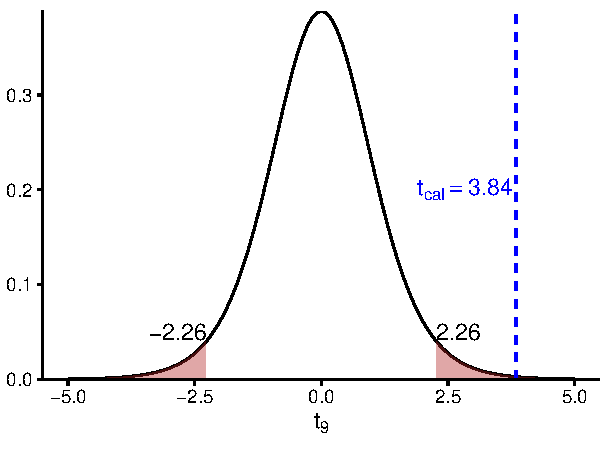
\includegraphics[width=\textwidth]{plots/single-mean-t-test.pdf}
                \end{center}
            \end{column}
        \end{columns}
    \end{frame}


    \section{Test about Two Means (Independent Samples)}


    \begin{frame}{Test about Two Means --- Choosing the Test}
        \begin{center}
            \small
            \begin{tabular}{p{8.5cm}lp{2.25cm}}
                \toprule
                \textbf{Criteria} & \textbf{Test} & \textbf{Sampling Distribution} \\
                \midrule
                $\sigma_1,\,\sigma_2$ known & $Z$ & $N(0,1)$ \\[0.6em]
                $\sigma_1,\,\sigma_2$ unknown but \textbf{equal} ($\sigma_1^2 = \sigma_2^2 = \sigma^2$),
                    $n \geqslant 30$ & $Z$ & $N(0,1)$ \\[0.6em]
                $\sigma_1,\,\sigma_2$ unknown but \textbf{equal},
                    $n < 30$ & $t$ & $t_{n_1+n_2-2}$ \\[0.6em]
                $\sigma_1,\,\sigma_2$ unknown and \textbf{unequal},
                    $n \geqslant 30$ & $Z$ & $N(0,1)$ \\[0.6em]
                $\sigma_1,\,\sigma_2$ unknown and \textbf{unequal},
                    $n < 30$ & $t$ & $t_{\nu}$ (Welch) \\
                \bottomrule
            \end{tabular}
        \end{center}
    \end{frame}


    \begin{frame}{Test about Two Means --- Test Statistics}
        \textbf{Equal variances} (pooled):
        \[
            S^2 = \frac{(n_1-1)S_1^2 + (n_2-1)S_2^2}{n_1+n_2-2},
            \qquad
            t_{\text{cal}} = \frac{\bar{x}_1 - \bar{x}_2}{S\sqrt{\tfrac{1}{n_1}+\tfrac{1}{n_2}}}
            \sim t_{n_1+n_2-2}
        \]

        \vspace{0.8em}

        \textbf{Unequal variances} (Welch):
        \[
            t_{\text{cal}} = \frac{\bar{x}_1 - \bar{x}_2}{\sqrt{\tfrac{S_1^2}{n_1}+\tfrac{S_2^2}{n_2}}}
            \sim t_{\nu},
            \qquad
            \nu = \frac{\left(\tfrac{S_1^2}{n_1}+\tfrac{S_2^2}{n_2}\right)^2}
                       {\dfrac{\left(\tfrac{S_1^2}{n_1}\right)^2}{n_1-1}
                        +\dfrac{\left(\tfrac{S_2^2}{n_2}\right)^2}{n_2-1}}
        \]
    \end{frame}


    \begin{frame}{Two Means (Independent) --- Example}
        \textbf{Problem:} A sample of 9 bulbs from Company~A had a mean lifetime of
        1309\,hrs ($s_1 = 419$); a sample of 16 bulbs from Company~B had a mean of
        1205\,hrs ($s_2 = 390$).
        Do the two companies' bulbs differ significantly in mean lifetime?
        Use $\alpha = 0.05$. Assume \textbf{unequal} population variances.

        \vspace{0.8em}

        Let $\mu_1, \mu_2 = $ mean lifetimes of bulbs from Company A and B respectively.

        \[
            H_0: \mu_1 = \mu_2 \quad \text{vs} \quad H_A: \mu_1 \neq \mu_2
        \]


        \vspace{1em}
        Here, \textbf{Welch degrees of freedom:}
                \[
                    \nu = \frac{(S_1^2/n_1 + S_2^2/n_2)^2}
                               {\frac{(S_1^2/n_1)^2}{n_1-1}+\frac{(S_2^2/n_2)^2}{n_2-1}}
                    \approx 16
                \]
    \end{frame}


    \begin{frame}{Two Means (Independent, Unequal Variances) --- Solution}
        \begin{columns}
            \begin{column}{0.55\textwidth}
                Welch degrees of freedom: \(\nu \approx 16\)

                \vspace{0.5em}

                \textbf{Critical value:} $t_{0.025,\,16} = 2.12$

                \vspace{0.5em}

                \textbf{Test statistic:}
                \[
                    t_{\text{cal}} = \frac{1309 - 1205}{\sqrt{\tfrac{419^2}{9}+\tfrac{390^2}{16}}}
                    = 0.61
                \]

                \vspace{0.5em}

                \textbf{Decision:} Since $|t_{\text{cal}}| = 0.61 < 2.12$,
                we \textbf{fail to reject} $H_0$ at 5\% level of significance.
                There is no significant difference in the mean lifetimes.
            \end{column}
            \begin{column}{0.45\textwidth}
                % R code to generate the plot:
                % library(ggplot2)
                % df_val <- 16
                % t_crit <- qt(0.975, df_val)   # 2.12
                % t_cal  <- 0.61
                %
                % x  <- seq(-4, 4, length.out = 600)
                % dd <- data.frame(x = x, y = dt(x, df_val))
                %
                % ggplot(dd, aes(x, y)) +
                %   geom_line() +
                %   geom_area(data = subset(dd, x <= -t_crit),
                %             aes(x, y), fill = "firebrick", alpha = 0.4) +
                %   geom_area(data = subset(dd, x >=  t_crit),
                %             aes(x, y), fill = "firebrick", alpha = 0.4) +
                %   geom_vline(xintercept = t_cal, linetype = "dashed",
                %              colour = "steelblue") +
                %   annotate("text", x = t_cal + 0.1, y = 0.15,
                %            label = expression(t[cal] == 0.61),
                %            hjust = 0, colour = "steelblue") +
                %   annotate("text", x = -t_crit, y = 0.02,
                %            label = "-2.12", hjust = 1) +
                %   annotate("text", x =  t_crit, y = 0.02,
                %            label =  "2.12", hjust = 0) +
                %   labs(x = expression(t[16]), y = "") +
                %   theme_classic()
                %
                % ggsave("plots/two-mean-indep-unequal.pdf", width = 4, height = 3)
                \begin{center}
                    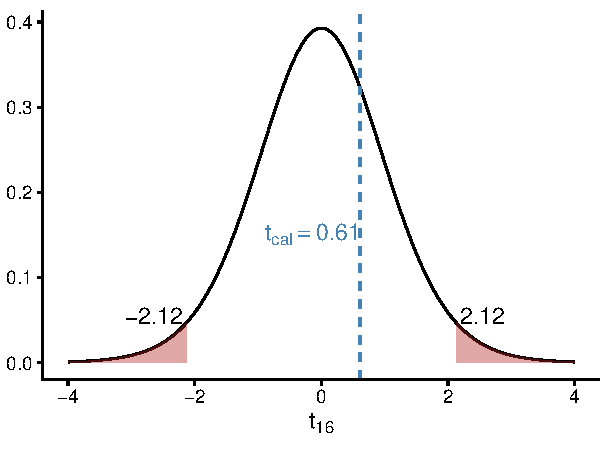
\includegraphics[width=\textwidth]{plots/two-mean-indep-unequal.pdf}
                \end{center}
            \end{column}
        \end{columns}
    \end{frame}


    \begin{frame}{Two Means (Independent, Equal Variances) --- Solution}
        \textbf{Same example, now assuming equal variances.}

        \vspace{0.5em}

        \textbf{Pooled variance:}
        \[
            S^2 = \frac{(n_1-1)S_1^2+(n_2-1)S_2^2}{n_1+n_2-2}
            = \frac{8\times 419^2 + 15\times 390^2}{23} = 160260.3
        \]

        \textbf{Test statistic:}
        \[
            t_{\text{cal}} = \frac{1309 - 1205}{S\sqrt{\tfrac{1}{9}+\tfrac{1}{16}}}
            = 0.197
        \]

        \textbf{Critical value:} $t_{0.025,\,23} = 2.069$

        \vspace{0.5em}

        \textbf{Decision:} Since $|t_{\text{cal}}| = 0.197 < 2.069$,
        we \textbf{fail to reject} $H_0$ at 5\% level of significance.
        There is no significant difference between the mean lifetimes of the two companies' bulbs.
    \end{frame}


    \section{Test about Two Means (Dependent Samples)}


    \begin{frame}{Test about Two Means --- Dependent (Paired) Samples}
        \begin{itemize}
            \item Used when the two samples are \textbf{not independent}
            \item Common when the same subjects are measured \textbf{before and after}
                a treatment, or under two conditions
            \item Define the \textbf{difference}: $d_i = x_i - y_i$
            \item This reduces the two-sample problem to a \textbf{one-sample}
                $t$-test on the differences
        \end{itemize}

        \vspace{0.5em}

        \textbf{Test statistic:}
        \[
            t_{\text{cal}} = \frac{\bar{d}}{s_d/\sqrt{n}} \sim t_{n-1}
            \quad \text{under } H_0
        \]

        where $\bar{d} = \frac{\sum d_i}{n}$ and
        $s_d^2 = \frac{1}{n-1}\left(\sum d_i^2 - \frac{(\sum d_i)^2}{n}\right)$
    \end{frame}


    \begin{frame}{Two Means (Dependent) --- Example}
        \textbf{Problem:} Nine adults agreed to test a new diet program.
        Their weights (in lb) were recorded before and after the program.
        Test whether the program is effective in reducing weight at $\alpha = 0.05$.

        \vspace{0.5em}

        \begin{center}
            \small
            \begin{tabular}{lccccccccc}
                \toprule
                & \multicolumn{9}{c}{\textbf{Adult}} \\
                \cmidrule{2-10}
                & 1 & 2 & 3 & 4 & 5 & 6 & 7 & 8 & 9 \\
                \midrule
                Before ($x_i$) & 132 & 138 & 126 & 114 & 122 & 132 & 142 & 119 & 137 \\
                After  ($y_i$) & 134 & 141 & 118 & 116 & 114 & 132 & 145 & 123 & 135 \\
                $d_i = x_i - y_i$ & $-2$ & $-3$ & $8$ & $-2$ & $8$ & $0$ & $-3$ & $-4$ & $2$ \\
                \bottomrule
            \end{tabular}
        \end{center}

        \[
            H_0: \mu_d = 0 \quad \text{vs} \quad H_A: \mu_d > 0
        \]
    \end{frame}


    \begin{frame}{Two Means (Dependent) --- Solution}
        \begin{columns}
            \begin{column}{0.55\textwidth}
                \textbf{Summary statistics:}
                \(
                    \bar{d} = \frac{4}{9} = 0.44, \qquad s_d^2 = 21.53
                \)

                \vspace{0.25em}

                \textbf{Test statistic:}
                \[
                    t_{\text{cal}} = \frac{0.44}{4.64/\sqrt{9}} = 0.28
                \]

                \textbf{Critical value:} $t_{0.05,\,8} = 1.86$

                \vspace{0.25em}

                \textbf{Decision:} Since $t_{\text{cal}} = 0.28 < 1.86$,
                we \textbf{fail to reject} $H_0$ at 5\% level of significance.

                \vspace{0.25em}

                \textbf{Conclusion:} There is insufficient evidence to conclude
                that the new diet program reduces weight.
            \end{column}
            \begin{column}{0.45\textwidth}
                % R code to generate the plot:
                % library(ggplot2)
                % df_val <- 8
                % t_crit <- qt(0.95, df_val)   # 1.86 (right-tailed)
                % t_cal  <- 0.28
                %
                % x  <- seq(-4, 4, length.out = 600)
                % dd <- data.frame(x = x, y = dt(x, df_val))
                %
                % ggplot(dd, aes(x, y)) +
                %   geom_line() +
                %   geom_area(data = subset(dd, x >= t_crit),
                %             aes(x, y), fill = "firebrick", alpha = 0.4) +
                %   geom_vline(xintercept = t_cal, linetype = "dashed",
                %              colour = "steelblue") +
                %   annotate("text", x = t_cal + 0.1, y = 0.20,
                %            label = expression(t[cal] == 0.28),
                %            hjust = 0, colour = "steelblue") +
                %   annotate("text", x = t_crit, y = 0.02,
                %            label = "1.86", hjust = 0) +
                %   labs(x = expression(t[8]), y = "") +
                %   theme_classic()
                %
                % ggsave("plots/paired-t-test.pdf", width = 4, height = 3)
                \begin{center}
                    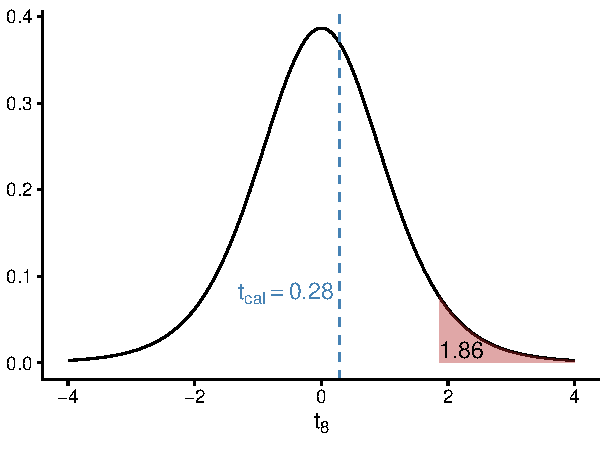
\includegraphics[width=\textwidth]{plots/paired-t-test.pdf}
                \end{center}
            \end{column}
        \end{columns}
    \end{frame}


    \section{Test about Several Means (ANOVA)}


    \begin{frame}{One-Way ANOVA --- Overview}
        \begin{itemize}
            \item Used to compare \textbf{more than two} population means simultaneously
            \item Hypotheses:
            \[
                H_0: \mu_1 = \mu_2 = \cdots = \mu_k
                \quad \text{vs} \quad
                H_A: \text{at least two means are unequal}
            \]
            \item The idea: decompose total variability into variability
                \emph{between groups} and \emph{within groups}
            \[
                \underbrace{\text{TSS}}_{\text{Total}} =
                \underbrace{\text{SSD}}_{\text{Between groups}} +
                \underbrace{\text{SSE}}_{\text{Within groups (error)}}
            \]
            \item \textbf{Assumptions:} $k$ independent random samples from
                $k$ normal populations with means $\mu_i$ and a \textbf{common variance}
                $\sigma^2$
        \end{itemize}
    \end{frame}


    \begin{frame}{One-Way ANOVA --- Test Statistic and ANOVA Table}
        \textbf{Test statistic:}
        \[
            F_{\text{cal}} = \frac{\text{MSD}}{\text{MSE}}
            = \frac{\text{SSD}/(k-1)}{\text{SSE}/(n-k)}
            \sim F_{k-1,\;n-k} \quad \text{under } H_0
        \]

        \vspace{0.5em}

        \textbf{ANOVA table:}
        \begin{center}
            \begin{tabular}{lcccc}
                \toprule
                \textbf{Source} & \textbf{df} & \textbf{SS} & \textbf{MS} & \textbf{F} \\
                \midrule
                Between groups & $k-1$ & SSD & $\text{MSD} = \text{SSD}/(k-1)$ &
                    $\text{MSD}/\text{MSE}$ \\
                Within groups (Error) & $n-k$ & SSE & $\text{MSE} = \text{SSE}/(n-k)$ & \\
                Total & $n-1$ & TSS & & \\
                \bottomrule
            \end{tabular}
        \end{center}
    \end{frame}


    \begin{frame}{ANOVA --- Computational Formulae}
        Let $n = \sum_{i=1}^k n_i$, $G = \sum_i \sum_j x_{ij}$,
        and $T_i = \sum_j x_{ij}$ (total for group $i$).

        \vspace{0.5em}

        \textbf{Correction term:}
        \[
            CT = \frac{G^2}{n}
        \]

        \textbf{Total sum of squares:}
        \[
            \text{TSS} = \sum_i \sum_j x_{ij}^2 - CT
        \]

        \textbf{Sum of squares between groups:}
        \[
            \text{SSD} = \sum_{i=1}^{k} \frac{T_i^2}{n_i} - CT
        \]

        \textbf{Sum of squares within groups (error):}
        \[
            \text{SSE} = \text{TSS} - \text{SSD}
        \]
    \end{frame}


    \begin{frame}{One-Way ANOVA --- Example}
        \textbf{Problem:} Random samples of students are selected from four
        departments (GE, AS, EEE, BA) of a university. Their marks are recorded
        below. Do the data indicate a significant difference in mean marks across
        departments? Use $\alpha = 0.05$.

        \begin{center}
            \small
            \begin{tabular}{ccccc}
                \hline
                & \textbf{GE} & \textbf{AS} & \textbf{EEE} & \textbf{BA} \\
                \hline
                & 80 & 70 & 67 & 81 \\
                & 74 & 64 & 66 & 60 \\
                & 84 & 70 & 60 & 50 \\
                & 89 & 78 & 68 & -- \\
                & 86 & 80 & -- & -- \\
                & 87 & -- & -- & -- \\
                & 77 & -- & -- & -- \\
                \hline
                $n_i$ & 7 & 5 & 4 & 3 \\
                $T_i$ & 577 & 282 & 341 & 191 \\
                \hline
            \end{tabular}
        \end{center}

        \[
            H_0: \mu_1 = \mu_2 = \mu_3 = \mu_4
            \quad \text{vs} \quad
            H_A: \text{at least two means are unequal}
        \]
    \end{frame}


    \begin{frame}{One-Way ANOVA --- Solution}
        \textbf{Calculations:} $n = 19$, $G = 1391$

        \(
            CT = \frac{1391^2}{19} = 101835.84
        \)

        \(
            \text{TSS} = (80^2 + 74^2 + \cdots + 50^2) - CT = 2021.16
        \)
        \(
            \text{SSD} = \frac{577^2}{7}+\frac{282^2}{4}+\frac{341^2}{5}+\frac{191^2}{3} - CT
            = 1022.98
        \)
        \(
            \text{SSE} = 2021.16 - 1022.98 = 998.18
        \)

        \begin{center}
            \begin{tabular}{lcccc}
                \toprule
                \textbf{Source} & \textbf{df} & \textbf{SS} & \textbf{MS} & \textbf{F} \\
                \midrule
                Department & 3 & 1022.98 & 340.99 & \textbf{5.12} \\
                Error & 15 & 998.18 & 66.55 & \\
                Total & 18 & 2021.16 & & \\
                \bottomrule
            \end{tabular}
        \end{center}

        \textbf{Critical value:} $F_{0.05,\,3,\,15} = 3.29$. Since $F_{\text{cal}} = 5.12 > 3.29$,
        we \textbf{reject} $H_0$. Mean marks differ significantly across departments.
    \end{frame}


    \section{Test about a Single Proportion}


    \begin{frame}{Test about a Single Proportion}
        \begin{itemize}
            \item Used when interest is in testing a claim about a population proportion $\pi$
            \item \textbf{Assumption:} large sample ($n > 30$); sample taken from
                a binomial population
            \item Let $p = x/n$ be the sample proportion
            \item \textbf{Test statistic:}
            \[
                Z_{\text{cal}} = \frac{p - \pi_0}{\sqrt{\pi_0(1-\pi_0)/n}}
                \sim N(0,1) \quad \text{under } H_0
            \]
            \item The hypotheses follow the same three forms (two-tailed, left-tailed,
                right-tailed) as for tests about a mean
        \end{itemize}
    \end{frame}


    \begin{frame}{Test about a Single Proportion --- Example}
        \textbf{Problem:} A nutritionist claims that at most 75\% of pre-school
        children in a certain country have a protein deficient diet.
        A survey of 300 children finds that 244 have protein deficiency.
        Is the claim justified at $\alpha = 0.01$?

        \vspace{0.8em}

        Let $\pi = $ proportion of children with protein deficient diet.

        \[
            H_0: \pi \leqslant 0.75 \quad \text{vs} \quad H_A: \pi > 0.75
        \]

        \vspace{0.5em}

        \textbf{Assumption:} Large sample ($n = 300 > 30$); binomial population.
    \end{frame}


    \begin{frame}{Test about a Single Proportion --- Solution}
        \begin{columns}
            \begin{column}{0.55\textwidth}
                \textbf{Sample proportion:}
                \(
                    p = \frac{244}{300} = 0.813
                \)

                \textbf{Test statistic:}
                \[
                    Z_{\text{cal}}
                    = \frac{0.813 - 0.75}{\sqrt{0.75 \times 0.25/300}}
                    = 2.52
                \]

                \textbf{Critical value:} $Z_{0.01} = 2.33$

                \vspace{0.5em}

                \textbf{Decision:} Since $Z_{\text{cal}} = 2.52 > 2.33$,
                we \textbf{reject} $H_0$ at 1\% level of significance.

                \vspace{0.5em}

                \textbf{Conclusion:} More than 75\% of pre-school children
                have a protein deficient diet.
            \end{column}
            \begin{column}{0.45\textwidth}
                % R code to generate the plot:
                % library(ggplot2)
                % z_crit <- qnorm(0.99)    # 2.326 (right-tailed)
                % z_cal  <- 2.52
                %
                % x  <- seq(-3.5, 4, length.out = 600)
                % df <- data.frame(x = x, y = dnorm(x))
                %
                % ggplot(df, aes(x, y)) +
                %   geom_line() +
                %   geom_area(data = subset(df, x >= z_crit),
                %             aes(x, y), fill = "firebrick", alpha = 0.4) +
                %   geom_vline(xintercept = z_cal, linetype = "dashed",
                %              colour = "blue") +
                %   annotate("text", x = z_cal + 0.05, y = 0.15,
                %            label = expression(Z[cal] == 2.52),
                %            hjust = 0, colour = "blue") +
                %   annotate("text", x = z_crit, y = 0.02,
                %            label = "2.33", hjust = 0) +
                %   labs(x = "Z", y = "") +
                %   theme_classic()
                %
                % ggsave("plots/single-proportion-z.pdf", width = 4, height = 3)
                \begin{center}
                    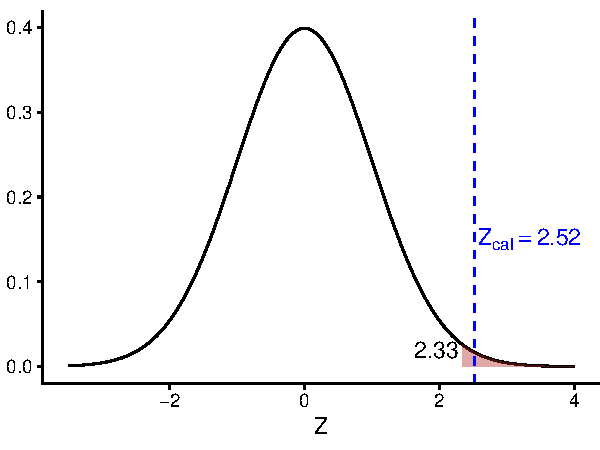
\includegraphics[width=\textwidth]{plots/single-proportion-z.pdf}
                \end{center}
            \end{column}
        \end{columns}
    \end{frame}


    \section{Test about Two Proportions}


    \begin{frame}{Test about Two Proportions}
        \begin{itemize}
            \item Used to compare proportions from two \textbf{independent} populations
            \item \textbf{Assumption:} both samples are large ($n_1, n_2 > 30$)
            \item Let $p_1 = x_1/n_1$ and $p_2 = x_2/n_2$ be the two sample proportions
            \item \textbf{Pooled proportion} (used when $H_0: \pi_1 = \pi_2$):
            \[
                p = \frac{x_1 + x_2}{n_1 + n_2}
            \]
            \item \textbf{Test statistic:}
            \[
                Z_{\text{cal}} = \frac{p_1 - p_2}{\sqrt{p(1-p)\left(\tfrac{1}{n_1}+\tfrac{1}{n_2}\right)}}
                \sim N(0,1) \quad \text{under } H_0
            \]
        \end{itemize}
    \end{frame}


    \begin{frame}{Test about Two Proportions --- Example}
        \textbf{Problem:} A mobile dealer sells Symphony and Walton.
        120 out of 200 customers prefer Symphony; 240 out of 500 prefer Walton.
        Can it be concluded at $\alpha = 0.05$ that Symphony is preferred over Walton?

        \vspace{0.8em}

        Let $\pi_s$ and $\pi_w$ be the proportions preferring Symphony and Walton.

        \[
            H_0: \pi_s = \pi_w \quad \text{vs} \quad H_A: \pi_s > \pi_w
        \]
    \end{frame}


    \begin{frame}{Test about Two Proportions --- Solution}
        \begin{columns}
            \begin{column}{0.55\textwidth}
                \textbf{Sample proportions:}
                \(
                    p_s = \frac{120}{200} = 0.60,
                    \quad
                    p_w = \frac{240}{500} = 0.48
                \)

                \vspace{0.5em}

                \textbf{Pooled proportion:}
                \(
                    p = \frac{120+240}{200+500} = \frac{360}{700} = 0.514
                \)

                \vspace{0.5em}

                \textbf{Test statistic:}
                \[
                    Z_{\text{cal}} =
                    \frac{0.60 - 0.48}{\sqrt{0.514 \times 0.486\left(\tfrac{1}{200}+\tfrac{1}{500}\right)}}
                    = 2.87
                \]

                \textbf{Critical value:} $Z_{0.05} = 1.64$

                \vspace{0.5em}

                \textbf{Decision:} Since $Z_{\text{cal}} = 2.87 > 1.64$,
                we \textbf{reject} $H_0$ at 5\% level of significance.
                Symphony is preferred over Walton.
            \end{column}
            \begin{column}{0.45\textwidth}
                % R code to generate the plot:
                % library(ggplot2)
                % z_crit <- qnorm(0.95)   # 1.645 (right-tailed)
                % z_cal  <- 2.87
                %
                % x  <- seq(-3.5, 4.5, length.out = 600)
                % df <- data.frame(x = x, y = dnorm(x))
                %
                % ggplot(df, aes(x, y)) +
                %   geom_line() +
                %   geom_area(data = subset(df, x >= z_crit),
                %             aes(x, y), fill = "firebrick", alpha = 0.4) +
                %   geom_vline(xintercept = z_cal, linetype = "dashed",
                %              colour = "blue") +
                %   annotate("text", x = z_cal + 0.05, y = 0.15,
                %            label = expression(Z[cal] == 2.87),
                %            hjust = 0, colour = "blue") +
                %   annotate("text", x = z_crit, y = 0.02,
                %            label = "1.64", hjust = 0) +
                %   labs(x = "Z", y = "") +
                %   theme_classic()
                %
                % ggsave("plots/two-proportion-z.pdf", width = 4, height = 3)
                \begin{center}
                    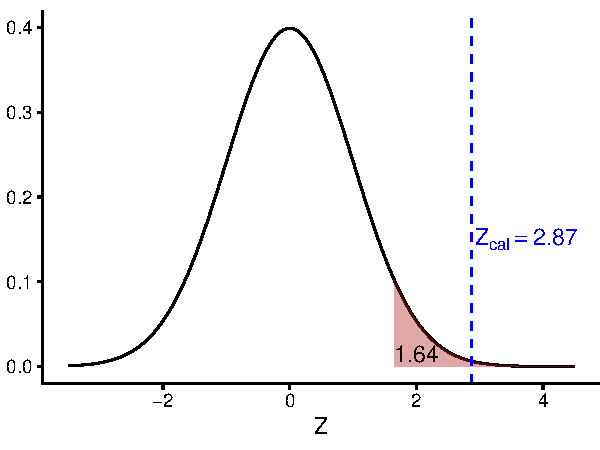
\includegraphics[width=\textwidth]{plots/two-proportion-z.pdf}
                \end{center}
            \end{column}
        \end{columns}
    \end{frame}


    \section*{Thank you.}

\end{document}